% Copyright 2007 by Till Tantau
%
% This file may be distributed and/or modified
%
% 1. under the LaTeX Project Public License and/or
% 2. under the GNU Public License.
%
% See the file doc/licenses/LICENSE for more details.



\documentclass{beamer}

%
% DO NOT USE THIS FILE AS A TEMPLATE FOR YOUR OWN TALKS�!!
%
% Use a file in the directory solutions instead.
% They are much better suited.
%


% Setup appearance:

\usetheme{Darmstadt}
\usefonttheme[onlylarge]{structurebold}
\setbeamerfont*{frametitle}{size=\normalsize,series=\bfseries}
\setbeamertemplate{navigation symbols}{}


% Standard packages

\usepackage[english]{babel}
\usepackage[utf8]{inputenc}
% \usepackage[latin1]{inputenc}
\usepackage{times}
\usepackage[T1]{fontenc}
\usepackage{listings}

% Setup TikZ

\usepackage{tikz}
\usetikzlibrary{shapes.gates.logic.US,trees,positioning,arrows}
\tikzstyle{block}=[draw opacity=0.7,line width=1.4cm]


% Author, Title, etc.

\title[How to create centralized user and assets database with LDAP] 
{%
  LDAP as user and assets directory
%
}

\author[Alex Kuklin]
{
  Alex Kuklin <alex@kuklin.ru> 
}

\institute[Varna Lab]
{
Varna Lab
}

\date[2011]
{2011}



% The main document

\begin{document}


\begin{frame}

Subjects:

\begin{itemize}
\item user database management (LDAP)
\item monitoring
\item backup
\item security and change management
\item virtualization with openVZ
\item VoIP
\end{itemize}


\end{frame}

\begin{frame}
  \titlepage
\end{frame}

\begin{frame}{Outline}
  \tableofcontents
\end{frame}


\section{What do we store}

\begin{frame}{User database in general}
For every multiuser system we need to maintain a user database. 

Different systems and applications use different ways to identify users and store different data.
\end{frame}

\begin{frame}[fragile]{Person, organization, etc}

\begin{itemize}
\item person
  \begin{itemize}
  \item person (sn cn userPassword telephoneNumber seeAlso description)
  \item organizationalPerson (title x121Address  registeredAddress  telephoneNumber   facsimileTelephoneNumber  street  ... )
  \item inetOrgPerson ( displayName givenName homePhone homePostalAddress mail mobile jpegPhoto uid userCertificate ... )
  \end{itemize}
\item organization (businessCategory registeredAddress telephoneNumber street postalAddress description ... )
\end{itemize}

\end{frame}

\begin{frame}{System accounts}
\begin{itemize}
\item Posix - used in unix-style systems; defined by rfc2307bis; numeric user and group ids 
\item Security Account Manager - used in MS Windows; Security identifier as unique id
\end{itemize}
\end{frame}


\begin{frame}[fragile]{Posix Account}
\begin{itemize}
\item Used in unix-style systems
\item Locally-unique uid/gid
\end{itemize}

Account sample:

\begin{verbatim}
uid: username
uidNumber: 10000
gidNumber: 10000
homeDirectory: /home/username
loginShell: /bin/bash
userPassword:: (encrypted password)
\end{verbatim}

\end{frame}

\begin{frame}[fragile]{SAM Account}
\begin{itemize}
\item Used in MSWindows systems
\item Globally-unique SID
\end{itemize}

Account sample:
\begin{verbatim}
uid: guest2
sambaSID: S-1-5-21-2447931902-1787058256-
  3961074038-5006
sambaPrimaryGroupSID: S-1-5-21-2447931902-
  1787058256-3961074038-513
sambaNTPassword: (encrypted password)
\end{verbatim}

\end{frame}

\begin{frame}[fragile]{SAM Account (continued)}

SID structure: S-1-5-21-3623811015-3361044348-30300820-1013 can be split down to:
\begin{itemize}
\item S The string is a SID.
\item 1 The revision level (the version of the SID specification).
\item 5  The identifier authority value.
\item 21-3623811015-3361044348-30300820  - domain or local computer identifier
\item 1013  - a Relative ID (RID). Any group or user that is not created by default will have a Relative ID of 1000 or greater.
\end{itemize}
\end{frame}

\begin{frame}[fragile]{Assets}

\begin{itemize}
\item computers
\item network devices
\item etc

\end{itemize}

\end{frame}

\section{How do we store}

\begin{frame}
\tableofcontents[currentsubsection]
\end{frame}


\subsection{Native ways}
\begin{frame}
\tableofcontents[currentsubsection]
\end{frame}

\begin{frame}

\begin{itemize}
\item Native linux-way -- passwd file, NIS.
\item Native windows-way -- registry, ActiveDirectory.
\item Databases
\end{itemize}
\end{frame}

\subsection{LDAP in brief}


\begin{frame}
\tableofcontents[currentsubsection]
\end{frame}

\begin{frame}{Concept}
\begin{itemize}
\item the utopic concept of global directory services - X.500 series standards
\item defined as a protocol for accessing direcory services via TCP/IP
\item Lightweight Directory Access \emph{Protocol} - more than a protocol now
\item local/corporate directories in our days 
\end{itemize}
\end{frame}

\begin{frame}{tree structure}
        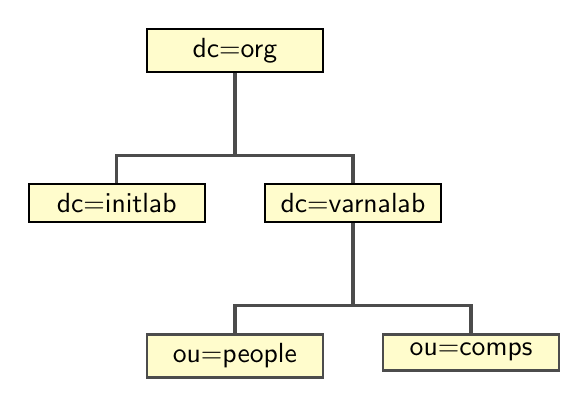
\begin{tikzpicture}[
    event/.style={rectangle,thick,draw,fill=yellow!20,text width=2cm,
		text centered,font=\sffamily,anchor=north},
    edge from parent/.style={very thick,draw=black!70},
    edge from parent path={(\tikzparentnode.south) -- ++(0,-1.05cm)
			-| (\tikzchildnode.north)},
    level 1/.style={sibling distance=3cm,level distance=1.4cm,
			growth parent anchor=south,nodes=event},
    level 2/.style={sibling distance=3cm},
    level 3/.style={sibling distance=2cm},
    level 4/.style={sibling distance=2cm}
]
    \node (g1) [event] {dc=org}
	     child{node [event] {dc=initlab} }
	     child{node  {dc=varnalab}
	     	child{node   {ou=people}}
	     	child{node   {ou=comps}}
 };
	
        \end{tikzpicture}

\end{frame}

\begin{frame}{flexible schemas}
\begin{itemize}
\item every object may belong to different object classes
\item schemas may be added to existing directory
\end{itemize}
\end{frame}

\begin{frame}{Distinguished Name}

dn: uid=user1, ou=people, dc=varnalab, dc=org

dn: cn=Ivan Petrov, ou=people, dc=varnalab, dc=org

\begin{itemize}
\item DN - unique identifier
\item different fields may be used in different situations (cn vs. uid) 
\end{itemize}

\end{frame}

\subsection{Why LDAP?}

\begin{frame}
\tableofcontents[currentsubsection]
\end{frame}

\begin{frame}{Well documented}

\begin{itemize}
      \item The Protocol [RFC4511]
      \item Directory Information Models [RFC4512]
      \item Authentication Methods and Security Mechanisms [RFC4513]
      \item String Representation of Distinguished Names [RFC4514]
      \item String Representation of Search Filters [RFC4515]
      \item Uniform Resource Locator [RFC4516]
      \item Syntaxes and Matching Rules [RFC4517]
      \item Internationalized String Preparation [RFC4518]
      \item Schema for User Applications [RFC4519]
\end{itemize}

\end{frame}

\begin{frame}{Well supported}
\begin{itemize}
\item almost any software dealing with user database have ldap access option
\end{itemize}
\end{frame}

\begin{frame}{Scalable}
\begin{itemize}
\item replication feature
\item referrals feature 
\end{itemize}
\end{frame}

\subsection{Software}

\begin{frame}{Servers}
\begin{itemize}
\item OpenLDAP
\item Mandriva Directory Server (MDS)
\item 389 Directory Server (RedHat/Fedora)
\item Novell eDirectory 
\item Sun Java System Directory Server
\item IBM Tivoli Directory Server
\item ... many other ...
\end{itemize}
\end{frame}



\begin{frame}{Management}
\begin{itemize}
\item phpldapadmin
\item luma - gui utility for accessing and managing LDAP database
\item lwat - LDAP Web-based Administration Tool
\item ldap-account-manager
\item GOsa
\end{itemize}
\end{frame}

\begin{frame}{GOsa management interface}
website: https://oss.gonicus.de/labs/gosa/

\includegraphics[width=100mm]{GOsa27-1.png}

\end{frame}

\begin{frame}{GOsa management interface}

\includegraphics[width=100mm]{GOsa27-2.png}

\end{frame}

\begin{frame}{ldap-utils}

Command line tools... for the brave

\end{frame}

\section{How do we access}

\begin{frame}[fragile]{LDAP search language}

RFC 2254 - just 8 pages? Hmmm....

\begin{description}
\item[filter]
(and(objectClass=posixAccount)(mailTo=*))
\item[searchbase] 
dn
\item[scope] 
base|one|sub|children
\item[dereference]  
never|always|search|find
\end{description}

Not relational!

Problem: no way to build complex queries.

\end{frame}

\begin{frame}{Password storage and check methods}

\begin{itemize}
\item password should be stored hashed
\item hash should not be published
\item cleartext password should not be transferred unencrypted
\item challenge-response authentication - poorly supported
\end{itemize}

\end{frame}

\begin{frame}{Linux user accounts}
\begin{itemize}
\item libnss-ldap - name service switch
\item libpam-ldap - pluggable auth module
\end{itemize}
\end{frame}

\begin{frame}{Samba server}
\begin{itemize}
\item configured in samba.conf 
\item ... worth separate speech
\end{itemize}
\end{frame}

\begin{frame}{Other}
\begin{itemize}
\item mail
\item asterisk
\item dns
\item dhcp
\end{itemize}
\end{frame}

\begin{frame}{Known problems}
\begin{itemize}
\item complex queries
\item isc dns/dhcp - no direct support
\end{itemize}
\end{frame}

\section{Conclusion}

\begin{frame}{1-2-3...}
How to try
\begin{itemize}
\item install openldap
\item install GOsa
\item create accounte
\item test it and use
\end{itemize}
\end{frame}

\end{document}


